\documentclass{beamer}
\usetheme[hideothersubsections]{AUTheme}
\setbeamertemplate{caption}[numbered]
\setbeamertemplate{bibliography item}[text]%,
\setbeamertemplate{footline}[frame number]

\usepackage[scaled]{helvet}

\usepackage{url}

\usepackage{tikz,pgf}
\usetikzlibrary{arrows}

\usepackage{epstopdf}
\usepackage{siunitx}
\usepackage{amsmath}
\usepackage{graphicx,subfigure}
\usepackage[maxcitenames = 1, mincitenames=1,backend=bibtex]{biblatex}
\usepackage{multicol}
% \usepackage{../sty/media9/media9}
% \usepackage[utf8]{inputenc}
\usepackage{hypcap}

% used for image citations
\usepackage[absolute,overlay]{textpos}

\hyphenation{op-tical net-works semi-conduc-tor}

\title[DRTK Driver Assistance]{An On-Line Visual Driver Aid for\\ Safe and Precise Convoy Following in\\ Visibility-Impaired Conditions}
\author[]{Robert Cofield, Scott Martin, David Bevly}
\date{September , 2013} 

\newcommand{\citeitem}[1]{
  \emph{\citeyear{#1}}--\Citeauthor*{#1}, \citetitle{#1}
}


\AtBeginSection[] {
  \begin{frame}<beamer>
    \frametitle{Section Outline}
    \tableofcontents[currentsection,hideallsubsections]
  \end{frame}
}

\bibliography{../bib/master.bib}

%%%%%%%%%%%%%%%%%%%%%%%%%%%%%%%%%%%%%%%%%%%%%%%%%%%%%%%%%%%%%%%%%%%%%%%%%%%%%%%%

\begin{document}

%% Title Slide %%
\frame{\titlepage}

%%%%%%%%%%%%%%%%
%% Motivation %%
%%%%%%%%%%%%%%%%

\section{Motivation}

  %% Military 
  \begin{frame}{Military Convoying}
    \begin{figure}
      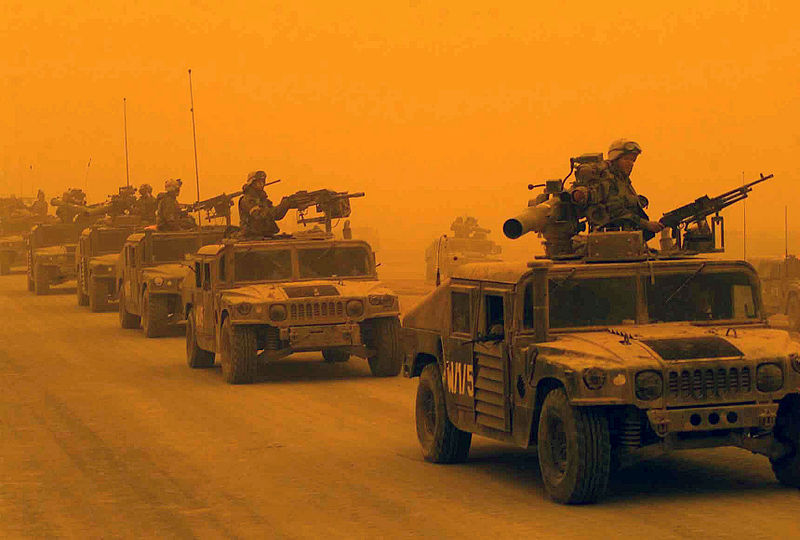
\includegraphics[width=5cm]{../graphics/convoy_sandstorm_orange.jpg}
      \caption{\cite{convoy_dust_orange}}
    \end{figure}
  \end{frame} 


%%%%%%%%%%%%%%%%%%%%%%%%%%%%%%%%
%% Literature & Previous Work %%
%%%%%%%%%%%%%%%%%%%%%%%%%%%%%%%%
\section{Literature}

  \subsection{DRTK}

    %% brief explanation
    \begin{frame}{Dynamic Base Real-Time Kinematic GNSS}
    \end{frame}

    %% LAMBDA
    \begin{frame}{LAMBDA Integer-Fixing Method}

    \end{frame}

    %% discuss accuracy
    \begin{frame}{Errors in DRTK}
    \end{frame}

  \subsection{TDCP}

    %% brief explanation
    \begin{frame}{Time-Differenced Carrier Phase GNSS}
    \end{frame}

    %% discuss accuracy
    \begin{frame}{Errors in TDCP}
    \end{frame}

  \subsection{Virtual Path}

    %% discuss virtual leader & path summation
    \begin{frame}{Construction of Path}
      \begin{figure}
        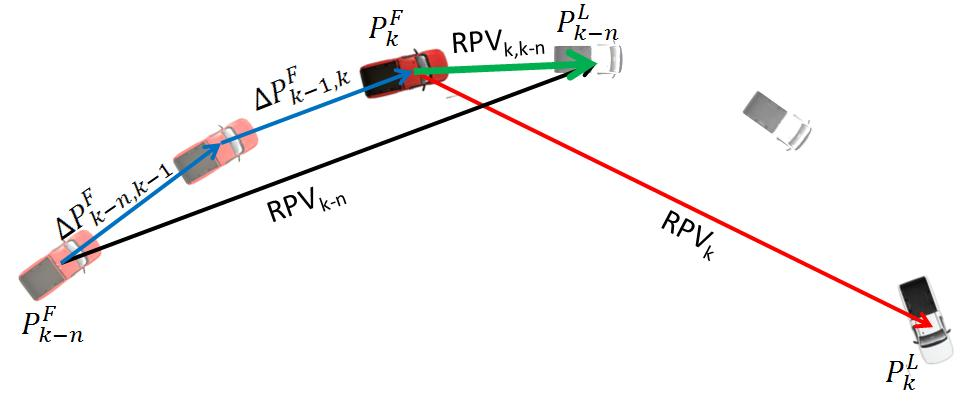
\includegraphics[width=10cm]{../graphics/path_algorithm.png}
      \end{figure}
    \end{frame}


%%%%%%%%%%%%%%%%%%%%%%%%%%%%%%%%%%%%
%% Presentation of final products %%
%%%%%%%%%%%%%%%%%%%%%%%%%%%%%%%%%%%%
\section{GUI}

  \subsection{Qt}

    \begin{frame}{Qt-Based GUI --- Data Display}
      \begin{figure}[ht] \centering
        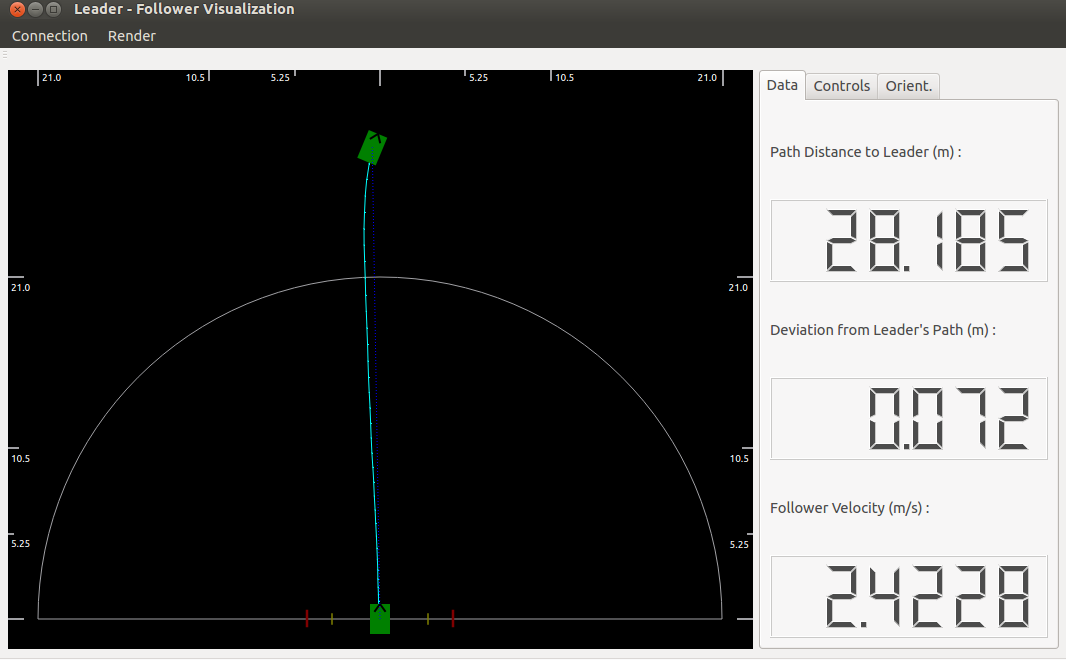
\includegraphics[width=4in] {../graphics/final_design_data.png}
        \caption{Qt GUI in normal operation} \label{fig:qt_data_display}
      \end{figure}
    \end{frame}

    \begin{frame}{Qt-Based GUI --- Controls}
      \begin{figure}[ht] \centering
        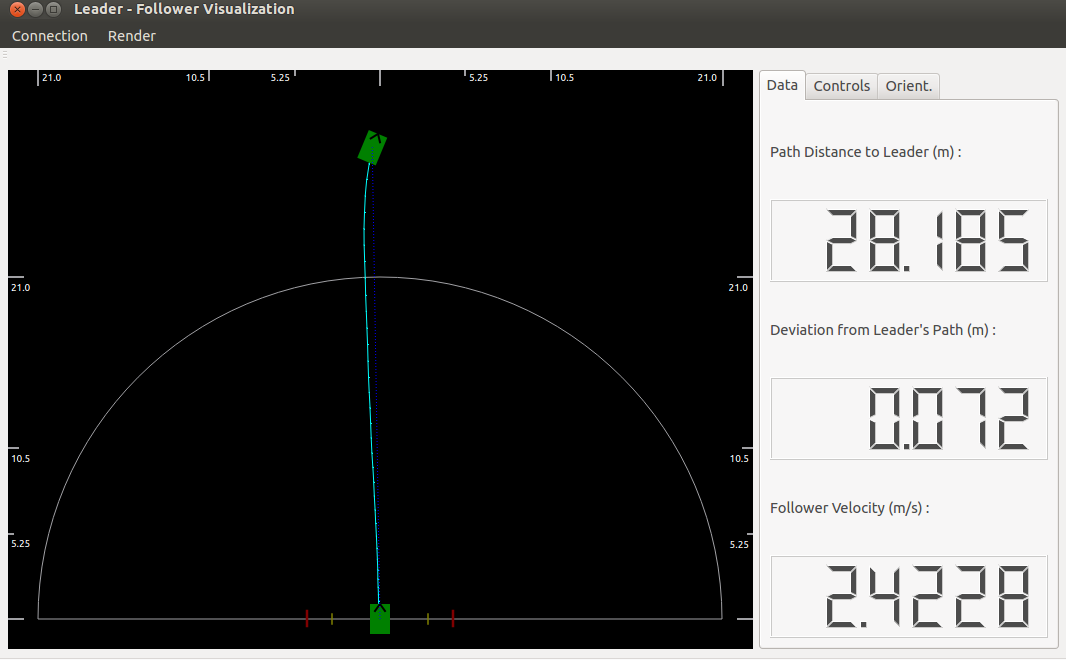
\includegraphics[width=4in] {../graphics/final_design_data.png}
        \caption{Qt GUI in normal operation} \label{fig:qt_controls}
      \end{figure}
    \end{frame}

  \subsection{Earth}

    \begin{frame}{Google Earth GUI --- Data Display}
    \end{frame}

    \begin{frame}{Google Earth GUI -- Controls}
    \end{frame}

  \subsection{Middleware}

    % talk about MOOS , etc
    \begin{frame}{Middleware}
    \end{frame}

    %% introduce interpolation
    \begin{frame}{Interpolation}
      \begin{figure}[ht] \centering
        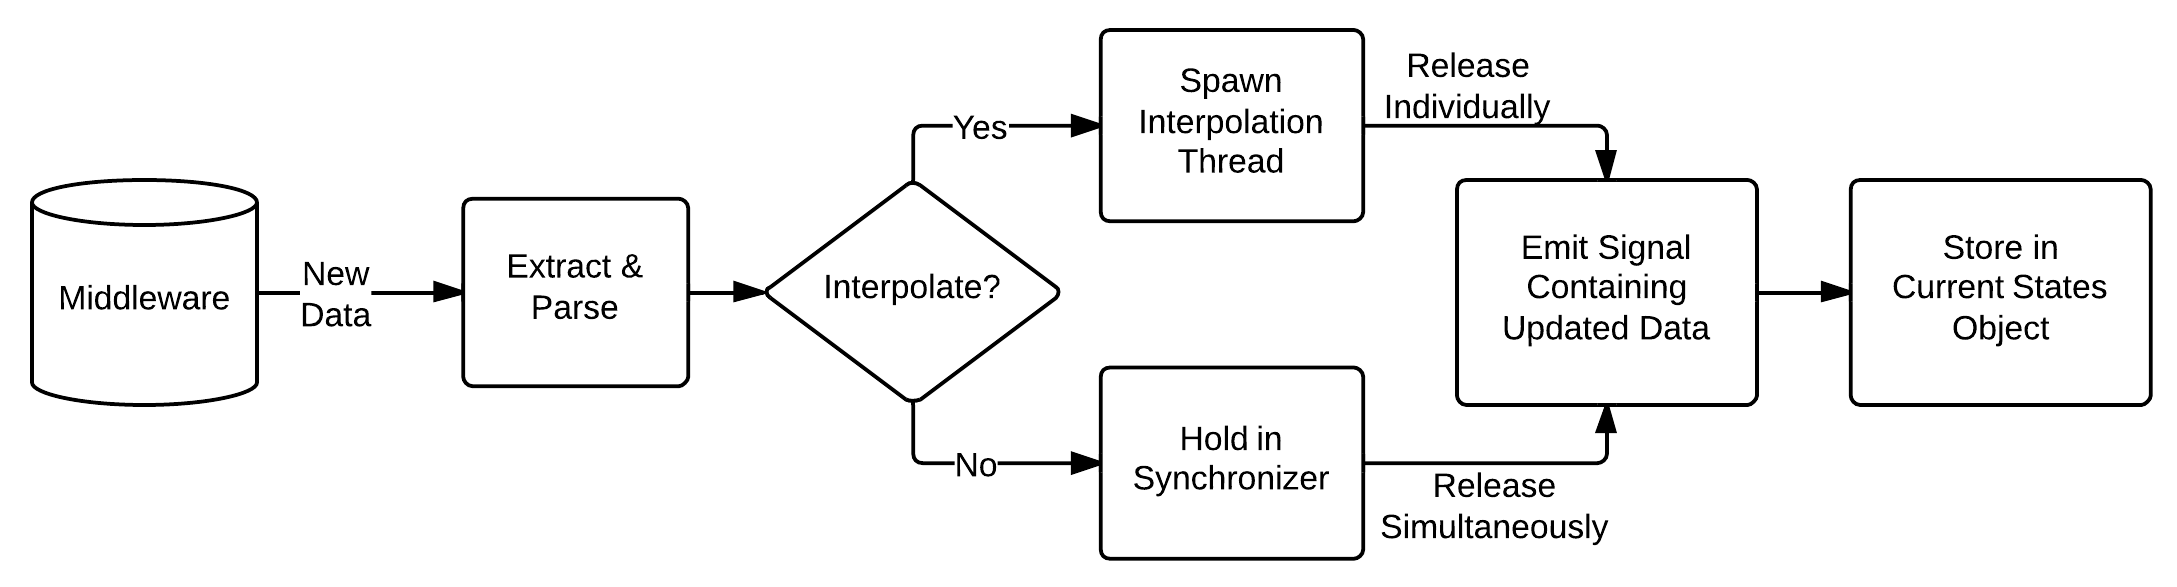
\includegraphics[width=5cm] {../graphics/middleware_diagram.png}
        \caption{Data input procedure} \label{fig:mw_diagram}
      \end{figure}
    \end{frame}


%%%%%%%%%%%%%%%%%%%%%%%%%%%%%%%%%%%
%% Tests that were run & Results %%
%%%%%%%%%%%%%%%%%%%%%%%%%%%%%%%%%%%
\section{Experimentation}

  \subsection{Hardware \& Setup}

    \begin{frame}{Leader Hardware}
      \begin{itemize}
        \item Novatel Propak v3 (OEMV board) L1/L2
        \item Pinwheel Antenna
        \item Digi Extend 900 Mhz radio
      \end{itemize}
    \end{frame}

    \begin{frame}{Follower Hardware}
      \begin{itemize}
        \item Novatel Propak v3 (OEMV board) L1/L2
        \item Pinwheel Antenna
        \item Digi Extend 900 Mhz radio
      \end{itemize}
    \end{frame}

    \begin{frame}{Presentation to Driver}
      \begin{figure}[ht] \centering
        \includegraphics[width=5cm] {../graphics/driver_view.jpg}
        \caption{View from the driver's seat} \label{fig:driver_view}
      \end{figure}
    \end{frame}


  \subsection{Testing Procedures}

    % Outline of tests
    \begin{frame}{Testing Procedures}
    
      Lane Change Test

      Precision Following Test
      
      Zero Landmark Test

    \end{frame}

    \begin{frame}{Lane Change Test}
      \begin{figure}
        % \documentclass[10pt]{article}
% \usepackage[utf8]{inputenc}
% \usepackage{pgf,tikz}
% \usetikzlibrary{arrows}
% \pagestyle{empty}
% \begin{document}

\definecolor{ttzzqq}{rgb}{0.2,0.6,0}
\definecolor{qqqqcc}{rgb}{0,0,0.8}
\definecolor{ffcctt}{rgb}{1,0.8,0.2}
\definecolor{ffzzqq}{rgb}{1,0.2,0}


\begin{tikzpicture}[
    scale=0.3,
    line cap=round,
    line join=round,
    >=triangle 45,
    x=1.0cm,y=1.0cm
    ]

    \begin{scope}[shift={(0,-15)}]

    \clip(-0.94,-2.06) rectangle (29.18,16.12);
    \draw [line width=5.2pt] (16,10)-- (2,10);
    \draw [line width=5.2pt] (16,14)-- (2,14);
    \draw [line width=5.2pt] (14,6)-- (16,6);
    % center stripe
    \draw [shift={(16,8)},line width=3pt,dash pattern=on 5pt off 5pt,color=ffcctt]  plot[domain=-1.57:1.57,variable=\t]({1*4*cos(\t r)+0*4*sin(\t r)},{0*4*cos(\t r)+1*4*sin(\t r)}); 
    \draw [line width=3pt,dash pattern=on 5pt off 5pt,color=ffcctt] (14,4)-- (16,4);
    \draw [line width=3pt,dash pattern=on 5pt off 5pt,color=ffcctt] (16,12)-- (4,12);

    \draw [shift={(16,8)},line width=5.2pt]  plot[domain=-1.57:1.57,variable=\t]({1*6*cos(\t r)+0*6*sin(\t r)},{0*6*cos(\t r)+1*6*sin(\t r)});
    \draw [shift={(16,8)},line width=5.2pt]  plot[domain=-1.57:1.57,variable=\t]({1*2*cos(\t r)+0*2*sin(\t r)},{0*2*cos(\t r)+1*2*sin(\t r)});
    \draw [line width=5.2pt] (16,2)-- (14,2);
    % path
    \draw [shift={(13.19,10.74)},line width=2pt,dotted,color=qqqqcc]  plot[domain=1.61:2.63,variable=\t]({1*2.58*cos(\t r)+0*2.58*sin(\t r)},{0*2.58*cos(\t r)+1*2.58*sin(\t r)});
    \draw [shift={(8.37,13.37)},line width=2pt,dotted,color=qqqqcc]  plot[domain=4.97:5.79,variable=\t]({1*2.91*cos(\t r)+0*2.91*sin(\t r)},{0*2.91*cos(\t r)+1*2.91*sin(\t r)});
    \draw [line width=2pt,dotted,color=qqqqcc] (13.08,13.32)-- (16.04,13.24);
    \draw [shift={(16,8.05)},line width=2pt,dotted,color=qqqqcc]  plot[domain=-1.58:1.56,variable=\t]({1*5.19*cos(\t r)+0*5.19*sin(\t r)},{0*5.19*cos(\t r)+1*5.19*sin(\t r)});

    \begin{scriptsize}
        % cones
        \fill [color=ffzzqq] (4,12)     circle (5.0pt);
        \fill [color=ffzzqq] (6,12)     circle (5.0pt);
        \fill [color=ffzzqq] (8,12)     circle (5.0pt);
        \fill [color=ffzzqq] (10,12)    circle (5.0pt);
        \fill [color=ffzzqq] (12,12)    circle (5.0pt);
        \fill [color=ffzzqq] (14,12)    circle (5.0pt);
        % leader
        \fill [color=ttzzqq,shift={(9.12,10.56)},rotate=90] (0,0) ++(0 pt,6.75pt) -- ++(5.85pt,-10.125pt)--++(-11.69pt,0 pt) -- ++(5.85pt,10.125pt);
        \draw[color=ttzzqq] (8,11) node {$Leader$};
        % follower
        \fill [color=ttzzqq,shift={(15.96,2.86)},rotate=270] (0,0) ++(0 pt,6.75pt) -- ++(5.85pt,-10.125pt)--++(-11.69pt,0 pt) -- ++(5.85pt,10.125pt);
        \draw[color=ttzzqq] (14.5,3.32) node {$Follower$};
    \end{scriptsize}

    \end{scope}

\end{tikzpicture}


% \end{document}
      \end{figure}
      % text describing test
    \end{frame}

    \begin{frame}{Precision Following Test}
      \begin{figure}
        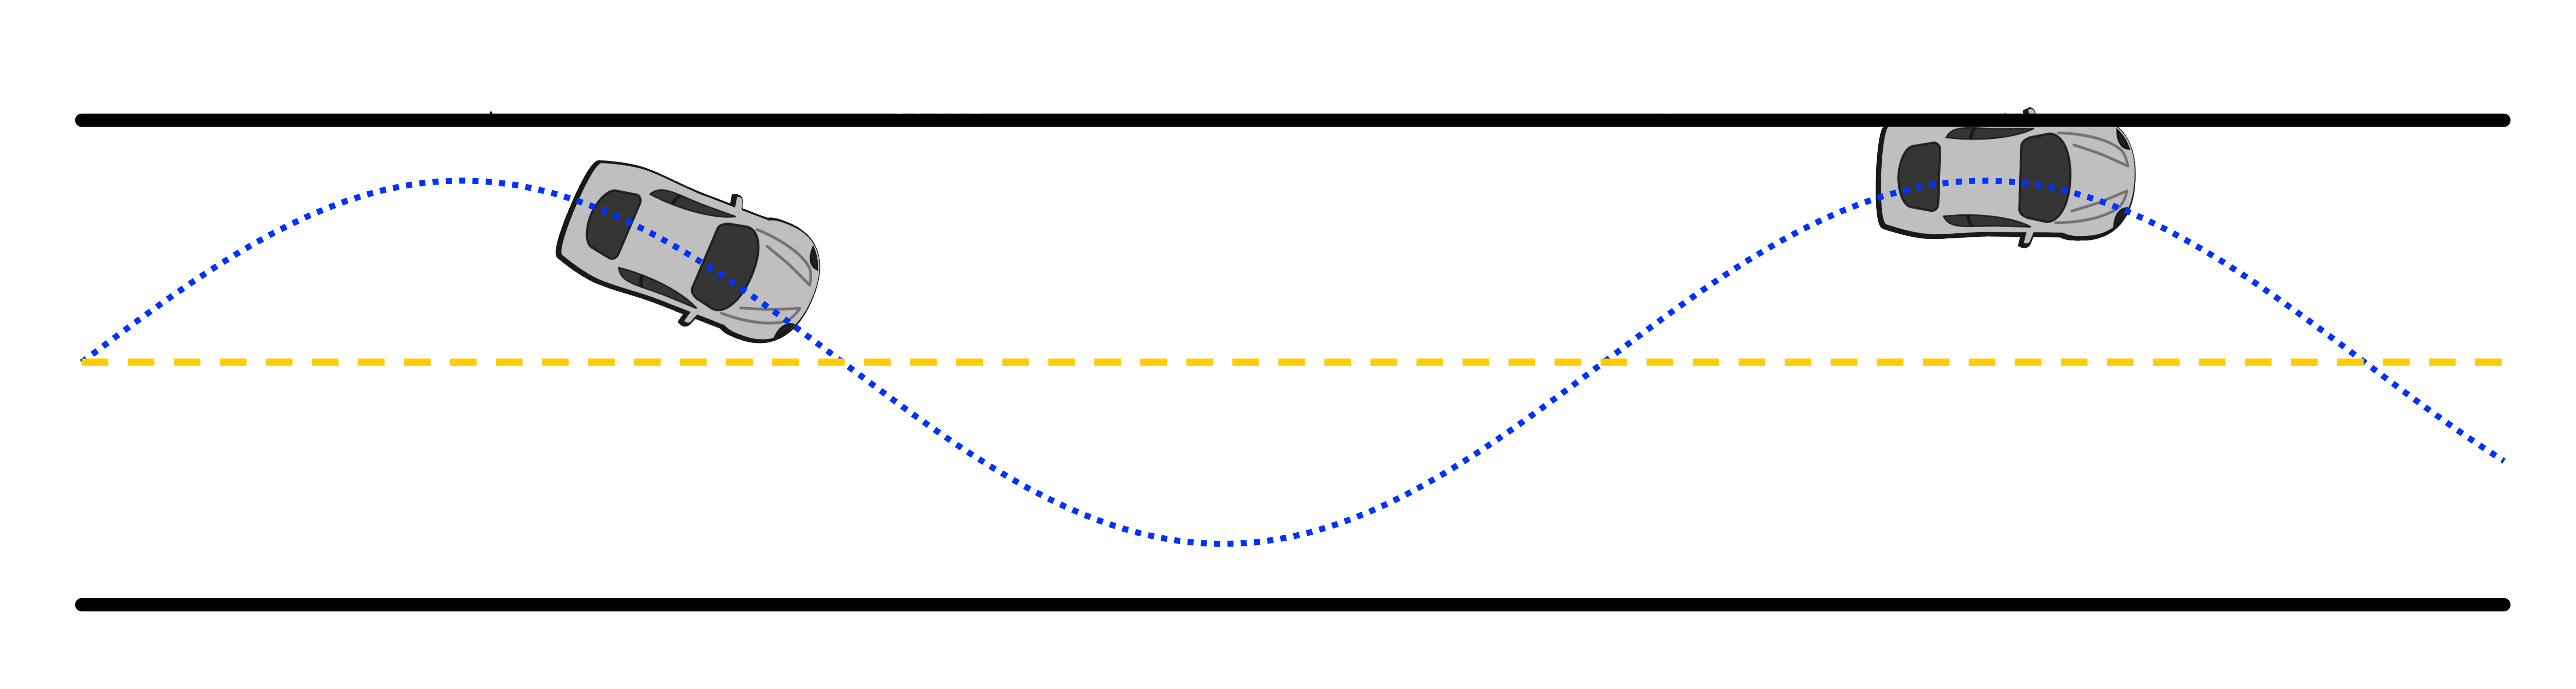
\includegraphics[width=10cm]{../graphics/precision_following_diagram.png}
      \end{figure}   
    \end{frame}

    \begin{frame}{Zero Landmark Test}
      \begin{figure}
        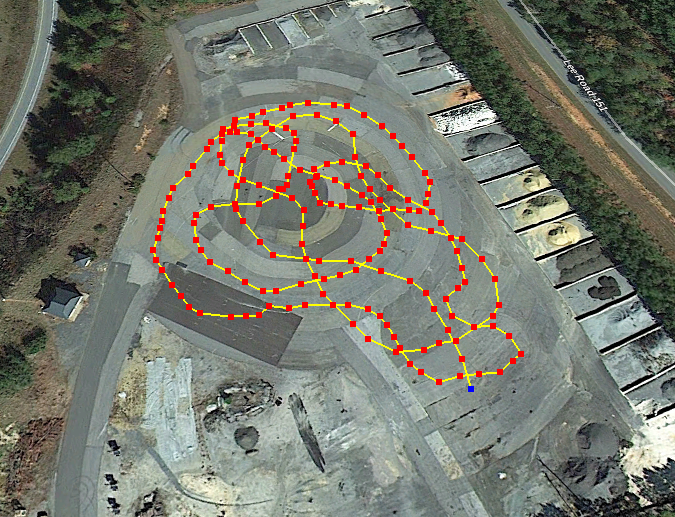
\includegraphics[width=7cm]{../graphics/zero_landmark_path.png}
      \end{figure}
    \end{frame}

  \subsection{Results}

  %%% Lane Change Test
    % What the drivers saw in each GUI during the lane change
    \begin{frame}{Driver View}
      \begin{figure}[ht] \centering
        \begin{minipage}[b]{0.45\linewidth} \centering 
          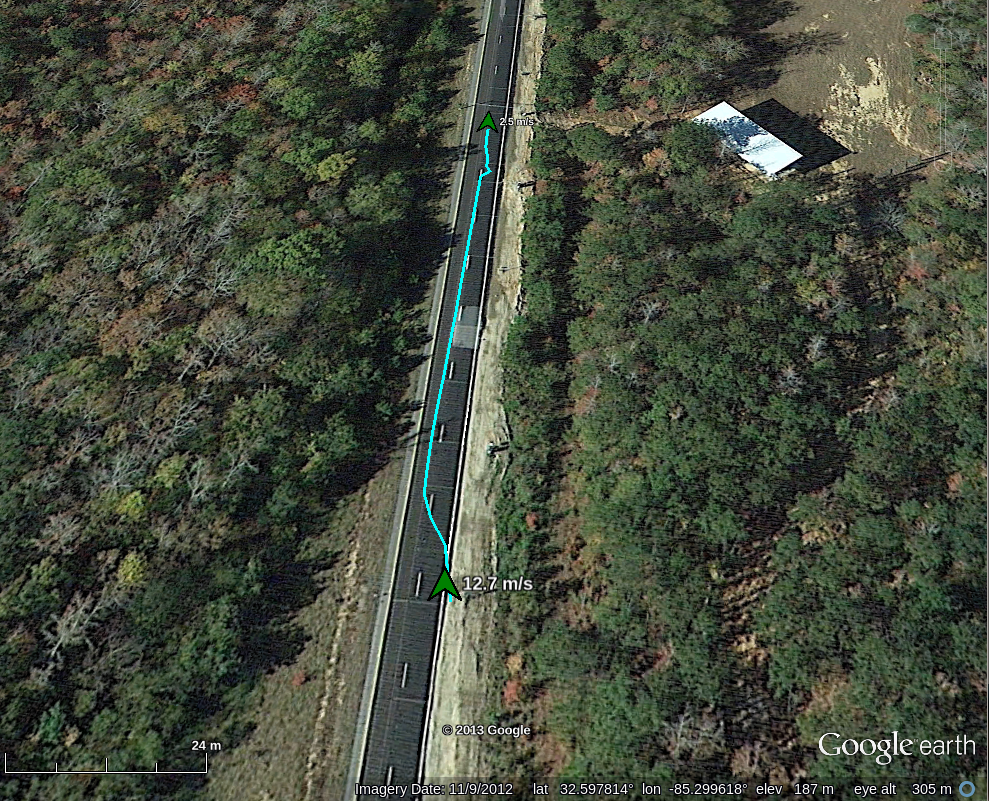
\includegraphics[width=\textwidth]{../graphics/lane_change.png}
          \caption{Google Earth GUI approaching the lane change maneuver}
        \end{minipage}
        \hspace{0.5cm}
        \begin{minipage}[b]{0.45\linewidth} \centering
          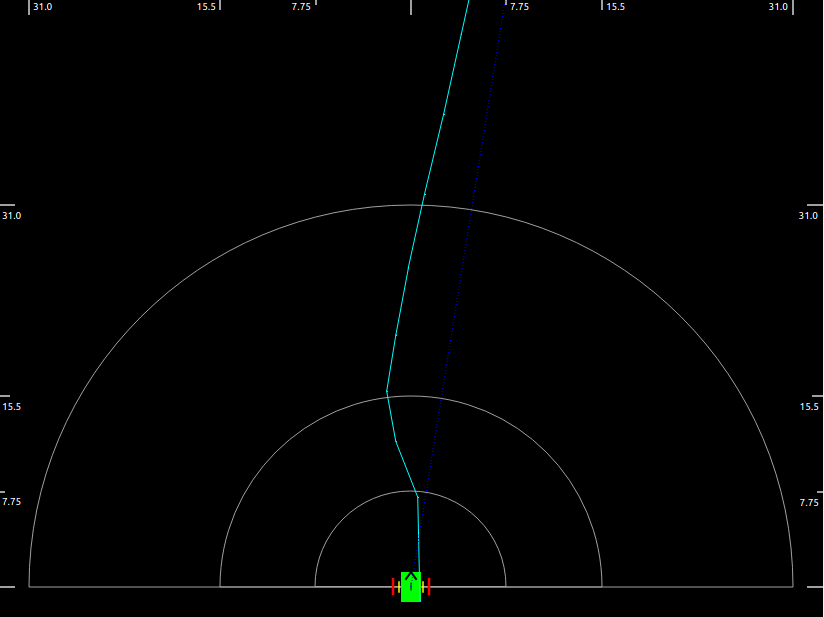
\includegraphics[width=\textwidth]{../graphics/lane_change_mono.png} 
          \caption{Qt GUI approaching the lane change maneuver}
        \end{minipage}
    \end{figure}
    \end{frame}

    % present data
    \begin{frame}{Lane Change Test --- Results}
    \end{frame}

    % what happened
    \begin{frame}{Lane Change Test --- Discussion}
    \end{frame}

  %%% Precision Following Test
    % present data
    \begin{frame}{Precision Following Test --- Results}
    \end{frame}

    % present data
    \begin{frame}{Precision Following Test --- Discussion}
    \end{frame}

  %%% Zero Landmark Test
    % present data
    \begin{frame}{Zero Landmark Test ---  Results}
    \end{frame}

    % what happened
    \begin{frame}{Zero Landmark Test ---  Discussion}
    \end{frame}


%%%%%%%%%%%%%%%%
%% Conclusion %%
%$%%%%%%%%%%%%%%
\section{Conclusion}

  \begin{frame}
  \end{frame}

\end{document}